\section{Histogram with Coarse Bins}
\label{sec:coarse bin histogram}

The one thing that slows the first histogram implementation is the need to have atomic increments for each bin.
Our idea is to split the bins into coarse bins so we have an estimate of how many integers will be in some range of bins.
The idea is illustrated in \cref{fig:coarse bins example}, where we have the sorted bin values at the top and the sorted coarse bin values at the bottom.

\begin{figure}[htb]
  \centering
  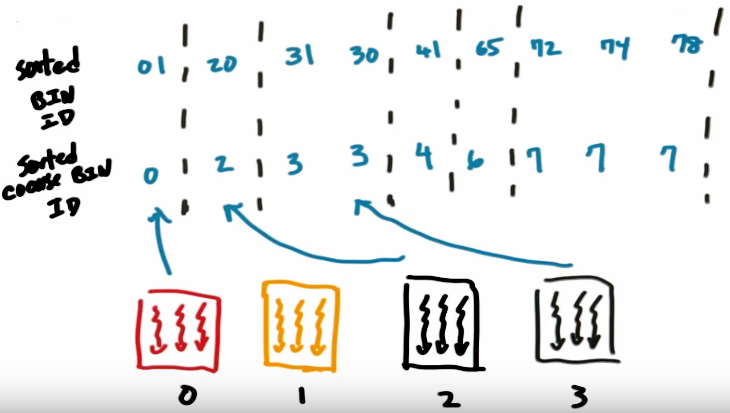
\includegraphics[width=.8\textwidth]{images/coarse-bin-example.png}
  \caption{Intuition behind coarse bin and kernel invokations}
  \label{fig:coarse bins example}
\end{figure}

Basically, the idea is still to use atomic increments but to divide them up into coarse bins so that they can be performed concurrently within the given range of coarse bins.
Consider \cref{fig:coarse bins example} where each coarse bin has a set of bins that fall into its category.
Each set in each bin is then executed by one kernel and divided into the correct bins.
So, the reasoning is that as a consequence of dividing the bin counting among more independent kernels the algorithm will run faster.

The proposed procedure runs as following
%
\begin{enumerate}
  \item Compute bin for each value
  \item Compute coarse bin for value
  \item Sort values w.r.t. the computed coarse bins
  \item Find starting position for each coarse bin
  \item For each coarse bin --- count each bin in given range
\end{enumerate}
%
We compute the bin for each respective value as presented in \cref{lst:value bin}, where \ttt{d\_in} is the list of values.

\begin{lstlisting}[caption={compute each value's bin}, label={lst:value bin}, numbers=none]
d_out[mid] = d_in[mid] % NUM_BINS;
\end{lstlisting}

Then the bins are divided into coarse bins as presented in \cref{lst:value coarse bin}, where the \ttt{d\_in} is the list of bins, i.e. the \ttt{d\_out} from \cref{lst:value bin}.

\begin{lstlisting}[caption={compute each value's coarse bin}, label={lst:value coarse bin}, numbers=none]
d_out[mid] = d_in[mid] / COARSE_SIZE;
\end{lstlisting}

We now have a list of values, their respective bins, and their coarse bins.
The next step is to sort all the values w.r.t. the coarse bins in ascending order, i.e. coarse bin 0 is first, followed by coarse bin 1, etc.
We use the radix sort implementation we developed earlier (with slight modifications to suite our needs) to perform the sorting based on the values in the list of coarse bins.

After the values have been sorted it is possible to find the starting positions of each coarse bin.
This gives us a starting value for each coarse bin from which it is possible to calculate how many values fall into each coarse bin.
We find the positions of the bins as presented in \cref{lst:coarse bin start} by running through each value and checking if the value before it was the same value.
If the previous value is not the same then we have a starting position for the next coarse bin.

\begin{lstlisting}[caption={find the start positions of each coarse bin}, label={lst:coarse bin start}, numbers=none]
if (d_in[mid] != d_in[mid-1])
  d_out[d_in[mid]] = mid;
\end{lstlisting}

Finally, the kernel responsible for counting and incrementing each bin for the histogram is invoked.
We invoke this kernel for each coarse bin, where we set the range in which the kernel should restrict its work.

\begin{lstlisting}[caption={kernel to do histogram count for each coarse bin}, label={lst:coarse histo kernel}]
__global__
void coarse_histogram_count(unsigned int* const d_out,
                            const unsigned int* const d_bins,
                            const unsigned int l_start,
                            const unsigned int l_end) {
  const unsigned int l_pos = l_start + threadIdx.x + blockIdx.x * blockDim.x;
  if (l_pos < l_start || l_pos >= l_end) return;

  const unsigned int bin = d_bins[l_pos];
  atomicAdd(&(d_out[bin]), 1);
}
\end{lstlisting}

We have that \ttt{l\_start} defines the starting index of the given coarse bin, and \ttt{l\_end} defines the maximum index for that coarse bin.
Together they define the range of which bins can be manipulates for each given kernel.

\subsection{Profiling and Analysis}

We tested and profiled our new implementation by using the \ttt{nvprof} command-line tools to get a file that could be imported into the NVIDIA Visual Profiler.
This is desirable because it is possible to run a guided analysis of the program.
The Visual Profiler runs analyses and informs what types of changes are recommended to try to maximise the usage of the GPU device.
We ran the code with

\begin{quote}
  \ttt{nvprof --analysis-metrics -o output-file.nvprof ./executable-to-test}
\end{quote}

which gave us a file that contained all the metrics needed for the guided analysis.
This file was opened with the NVIDIA Visual Profiler and the program performed analysis of how the GPU as used.
\Cref{fig:first impl} shows the output given by the NVIDIA Visual Profiler's initial GPU usage analysis.
It informs that the algorithm has low kernel concurrency and low compute utilisation.

\begin{figure}[htb]
  \centering
  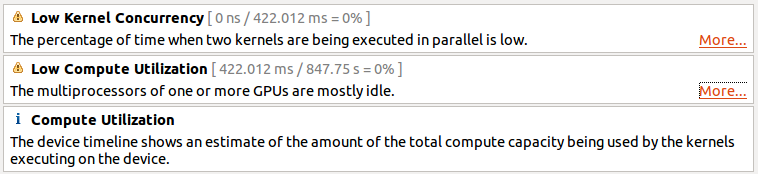
\includegraphics[width=.9\textwidth]{images/low-kernel-concurrency.png}
  \caption{NVIDIA Visual Profiler analysis}
  \label{fig:first impl}
\end{figure}

\subsection{Adding Streams}

It is possible to make kernel executions concurrent.
However, this only makes sense if the kernels are independent of each other.
So, if one or more kernels are not dependent of the output from the other kernels they can be executed concurrently.
In CUDA kernels are run concurrently with the use of streams.

Thus, from the visual profiler's analysis we tried to add streams to the kernels that were independent of the execution of the rest of the kernels.
This were the kernels that were in charge of counting and incrementing the final result of the histogram algorithm.
This modification to the code is presented in \cref{lst:coarse histo streams}.
We instantiate an array of streams, and for each iteration of the loop we create a stream and invoke the kernel with it.

\begin{lstlisting}[caption={Using streams to invoke kernels concurrently}, label={lst:coarse histo streams}]
// instantiate array of streams
cudaStream_t streams[COARSE_SIZE];

for (unsigned int i = 0; i < COARSE_SIZE; i++) {
  // create the stream for each kernel call
  cudaStreamCreate(&streams[i]);

  // set up range for local coarse bin
  local_bin_start = h_positions[i];
  local_bin_end   = (i == COARSE_SIZE-1) ? NUM_ELEMS : h_positions[i+1];

  // calculate local grid size
  amount = local_bin_end - local_bin_start;
  grid_size = amount / BLOCK_SIZE.x + 1;

  // make sure there is at least one value in coarse bin
  if (amount > 0)
    coarse_histogram_count<<<grid_size, BLOCK_SIZE, 0, streams[i]>>>(d_histogram, d_bins, local_bin_start, local_bin_end);
}
\end{lstlisting}


The resulting output did not boost the performance significantly.
We found that the sorting of the numbers used approximately $80\%$ of the execution time.
This means that the bottleneck was the sorting, and no longer the histogram's atomic increments.
The reason for the sorting being so slow may be because we use the Hillis and Steele scan in our radix sort implementation.
It might have made a difference to use Blelloch scan as it is more work efficient, which we presented in \cref{sec:workload and step size}.
